\subsection{Theoretische Grundlagen}
\subsection{Allgemeines zur Wärmekapazität}
Die spezifische Wärmekapazität, oder auch Molwärme, $c_{\text{mol}}$ ist nach der Thermodynamik wie folgt über die Wärmekapazität $C_{\text{V}}$ definiert:
\begin{equation*}
	c_{\text{mol}} = \frac{C_{\text{V}}}{n} = \frac{1}{n} \frac{\partial U}{\partial T} \bigg{\vert}_{V}.
\end{equation*}
\begin{center}
	\tiny{$n \, \widehat{=}$ Stoffmenge des Materials, $V \, \widehat{=}$ konstantes Volumen }
\end{center}
Allgemein wird ein Teil der zugeführten Wärme in Volumenarbeit (Ausdehnung) umgesetzt und die Wärmekapazitäten bei konstantem Volumen $C_{\text{V}}$ und bei konstantem Druck $C_{\text{p}}$ unterscheiden sich.
Festkörper dehnen sich weniger stark aus als Gase und die Wärmekapazitäten $C_{\text{V}}$ und $C_{\text{p}}$ sind im Festkörper annähernd gleich.
Die Wärmekapazität von Festkörpern wird hauptsächlich durch die Schwingung von Teilchen ausgemacht.
Es gibt jedoch auch einen elektronischen Teil der Wärmekapazität, der linear in T verläuft.
Gegen den Einfluss der schwingenden Teilchen ist die Wärmekapazität durch die freien Elektronen im Festkörper jedoch vernachlässigbar.

\subsection{Klassische Näherung}
Im Festkörper sind die Atome in gitterförmigen Kristallstrukturen angeordnet.
Die Temperatur eines Materials bedeutet mikroskopisch, dass die Atome in der Gitterstruktur schwingen und so Energie speichern.
Werden alle Teilchen im Festkörper als einzelne, unabhängige harmonische Oszillatoren genähert, wird von der klassischen Näherung gesprochen.
Die Energie eines Teilchens beträgt dann
\begin{equation*}
	U = \sum_{i=x,y,z} \bigg( \underbrace{ \,\,\, \frac{1}{2}mv_{\text{i}}^2 \,\,\, }_{\substack{\text{kin. Energie}}} + \underbrace{ \,\,\, \frac{1}{2} D i^2 \,\,\, }_{\substack{\text{pot. Energie}}} \bigg).
\end{equation*}
\begin{center}
	\tiny{$m \widehat{=}$ Masse des Teilchens, $v \widehat{=}$ Geschwindigkeit des Teilchens, $D \widehat{=}$ Kopplungskonstante (Federkonstante)}
\end{center}
Im klassischen Modell wird die Gesamtenergie der Atome durch das Äquipartitionstheorem statistisch zu gleichen Teilen zu kinetischer und potenzieller Energie aufgeteilt mit je $E_{\text{kin}} = E_{\text{pot}} = 1/2 k_{\text{B}} T $.
Die Gesamtenergie beträgt bei je drei Freiheitsgraden pro Teilchen und einer Teilchenanzahl $N$ entsprechend
\begin{equation*}
	U = 2 \cdot \frac{3}{2} N k_{\text{B}} T.
\end{equation*}
\begin{center}
	\tiny{$N\widehat{=}$ Teilchenzahl, $k_{\text{B}} \widehat{=}$ Boltzmann-Konstante, $T \widehat{=}$ Temperatur}
\end{center}
Somit liegt die Wärmekapazität $C_{\text{V}}$ bei
\begin{equation}
	C_{\text{V}} = \frac{\partial U}{\partial T} \bigg{\vert}_{V} = 3 N k_{\text{B}} = 3 R.
	\label{eqn:dulongpetit}
\end{equation}
\begin{center}
	\tiny{$R \widehat{=}$ Universelle Gaskonstante}
\end{center}
Dieser Zusammenhang wird \textit{Dulong-Petit-}Gesetz genannt.
Es beschreibt eine klassische Näherung der Schwingungen der Atome mit vielen verschiedenen Moden, also Phononen verschiedener Energien.
Bei Raumtemperatur und höheren Temperaturen passt dieses Modell zu den experimentellen Daten, bei niedrigen Temperaturen weichen Modell und Messdaten voneinander ab.

\FloatBarrier
\subsection{Einstein-Modell}
Die Quantisierungen der zuvor beschriebenen Gitterschwingungen werden \textit{Phononen} genannt.
Ein Phonon beschreibt also eine wellenförmige Anregung des Gitters mit einer zugeordeten Energie (eine Mode).
%Energie, also auch Frequenz $\omega$, hängen von der Wellenzahl $k$ ab.
%Dies ist die sognenannte Dispersionsrelation $\omega(k)$.
Phononen verschiedener Energien (verschiedene Moden) können sich überlagern.
Im Graph der Dispersionsrelation $\omega(k)$ (Abb. \ref{fig:disp}) lassen sich der \textit{optische} Zweig und der \textit{akustische} Zweig aus möglichen Phononen identifizieren.
Die optischen Phononen gilt näherungsweise $\omega(k) \approx \text{const.}$, während für die akustischen Phononen im Zentrum der Brillouin-Zone eher $\omega(k) \propto k $ gilt.
\begin{figure}[!ht]
	\centering
	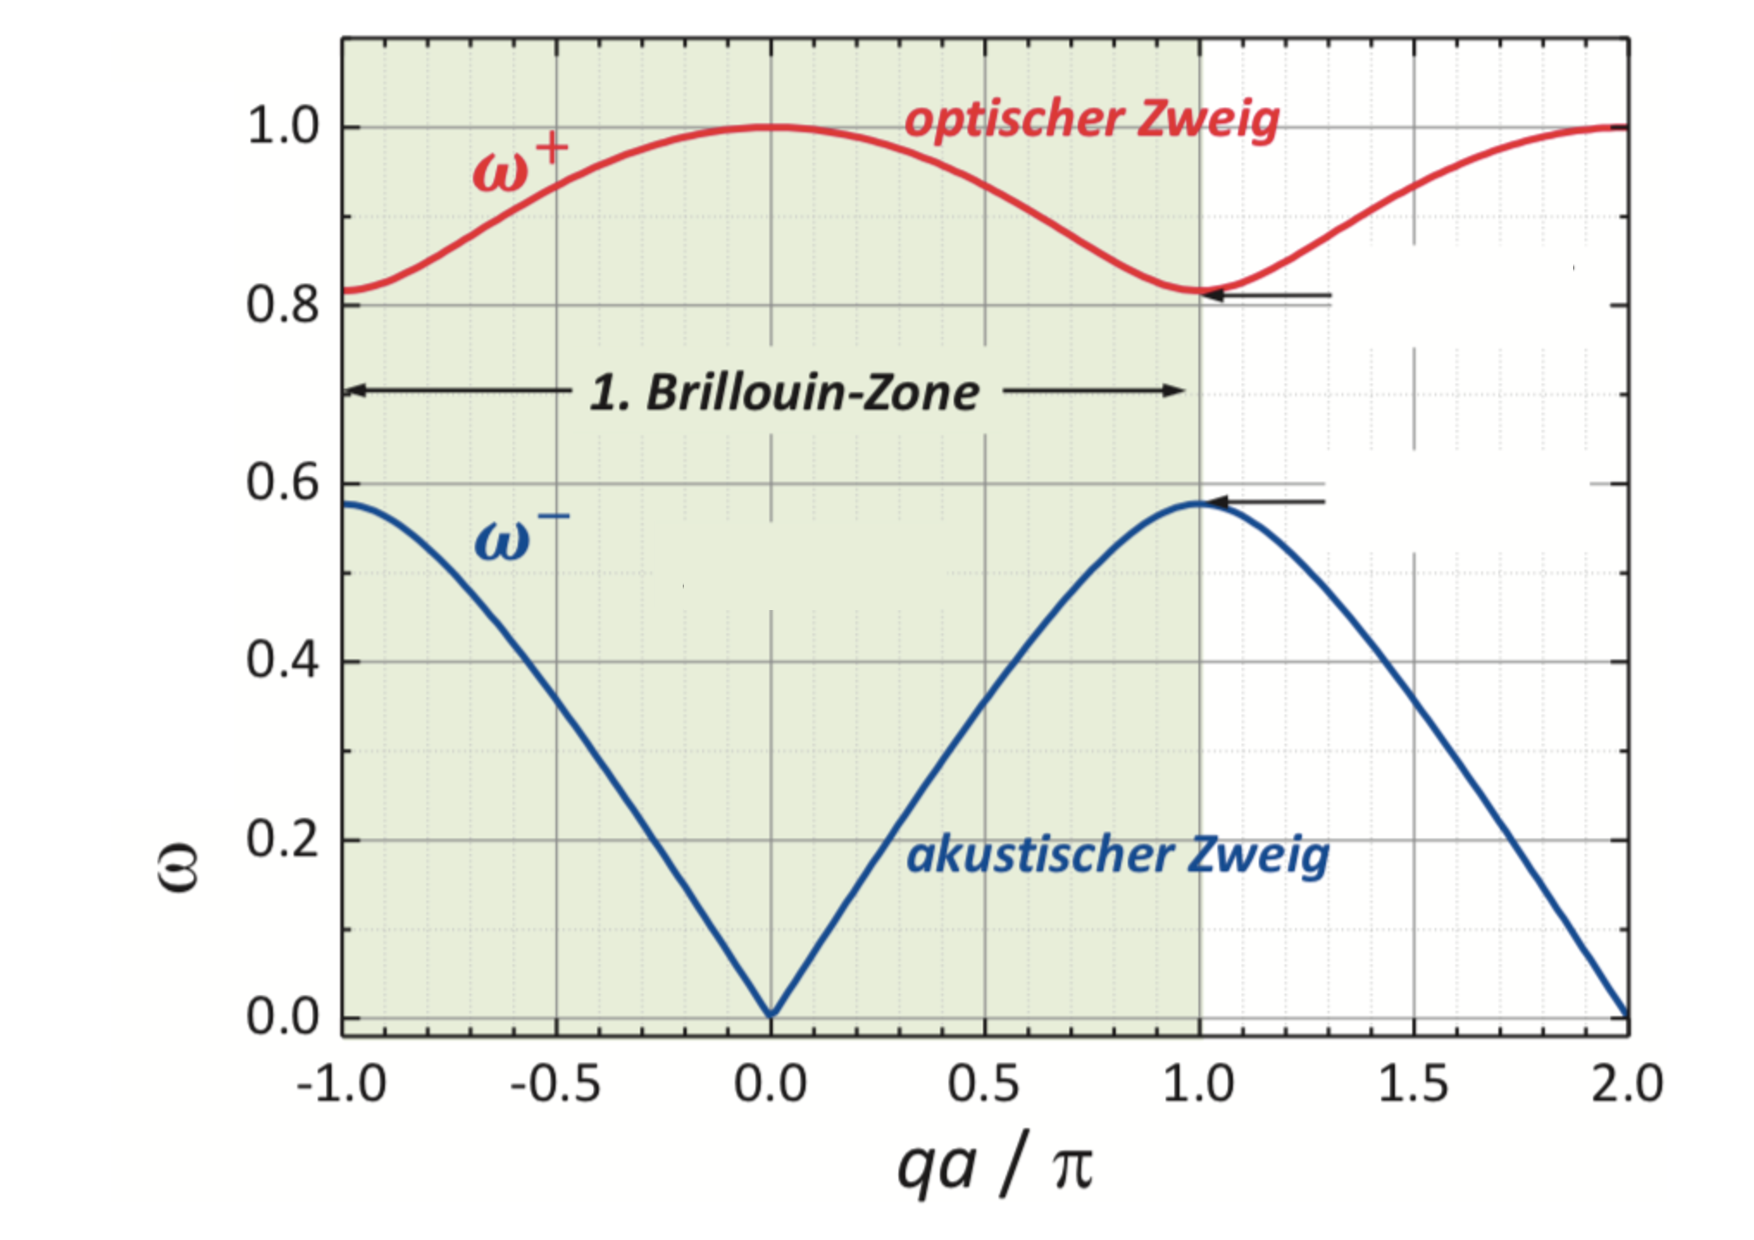
\includegraphics[width=0.75\textwidth]{content/images/phononen.pdf}
    \caption{Darstellungen der Dispersionsrelation einer zweiatomigen linearen Kette aus Atomen \cite{grossmarx}, modifiziert.}
    \label{fig:disp}
\end{figure}

Im Einstein-Modell wird angenommen, dass alle Phononen eine Energie (eine Mode) haben, also alle mit einer Frequenz $\omega_{\text{E}}$ schwingen.
Alle Teilchen liegen also im gleichen Zustand und die Zustandsdichte $D(\omega)$ ist entsprechend eine $\delta$-Funktion.
%Die Gesamtenergie der Teilchen im Gitter lässt sich mit einer Maxwell-Boltzmann-Verteilung der Besetzungszahl der Phononen berechnen:
%\begin{equation*}
%  U = \hbar \omega_\text{E} \langle n \rangle = \frac{1}{\exp\left(\frac{\hbar \omega_\text{E}}{k_\text{B} T}\right)-1}\,.
%\end{equation*}
Die mittlere Besetzungszahl $\langle n \rangle$ einer Mode berechnet sich über die Maxwell-Boltzmann-Verteilung:
\begin{equation*}
	\langle n \rangle = \frac{\exp{ \left( -\frac{\hbar \omega}{k_{\text{B}} T} \right)}}{ \sum_{n} \exp{\left( -\frac{\hbar \omega}{k_{\text{B}} T} \right)}} = \frac{1}{ \exp{ \left( \frac{\hbar \omega}{k_{\text{B}} T} \right)}-1}.
\end{equation*}
\begin{center}
	\tiny{$\hbar \widehat{=}$ reduziertes Plancksches Wirkungsquantum}
\end{center}
Der Erwartungswert für die Energie beträgt entsprechend für $N$ Teilchen mit 3 Freiheitsgraden:
\begin{equation*}
	\langle U \rangle = 3 N  \hbar \omega_{\text{E}} \langle n \rangle  = \frac{3 N k_{\text{B}} \hbar \omega_{\text{E}}}{\exp{\left( \frac{ \hbar \omega }{ k_{\text{B}} T } \right)} - 1}.
\end{equation*}

Für die Wärmekapazität gilt dann
\begin{equation*}
	C_{\text{V}} = \frac{\partial U}{\partial T} \bigg{\vert}_{V} = 3 N k_{\text{B}} \left( \frac{\hbar \omega}{k_{\text{B}} T} \right)^2
	\frac{ \exp{\left( \frac{ \hbar \omega }{ k_{\text{B}} T } \right)} }{ \left[ \exp{\left( \frac{ \hbar \omega }{ k_{\text{B}} T } \right)} - 1 \right]^2 } =
	3 N k_{\text{B}} \left( \frac{\hbar \omega}{k_{\text{B}} T} \right)^2
	\frac{ \exp{\left( \frac{ \Theta_{\text{E}} }{ T } \right)} }{ \left[ \exp{\left( \frac{ \Theta_{\text{E}} }{ T } \right)} - 1 \right]^2 }
\end{equation*}
mit der sogenannten Einstein-Temperatur
\begin{equation*}
	\Theta_{\text{E}} = \frac{\hbar \omega_{\text{E}}}{k_{\text{B}}}.
\end{equation*}

Für große Temperaturen ($T \gg \Theta_{\text{E}}$) ergibt sich über die Taylor-Entwicklung der Exponentialfunktion das Dulong-Petit-Gesetz (Gleichung \eqref{eqn:dulongpetit}).
Die Einstein-Temperatur ist somit durch die Schwingungsfrequenz $\omega$ eine materialabhängige Konstante.
Durch die Annahme, dass nur eine Mode vorhanden ist, entspricht das Modell bei sehr tiefen Temperaturen und geringen Frequenzen nicht der Realität.
Das Einstein-Modell passt jedoch sehr gut zu Anregungen mit optischen Phononen.

\subsection{Debye-Modell}
Das Debye-Modell geht von einer linearen Zustandsdichte $D(\omega) \propto \omega$ aus.
Die Phononen haben also eine kontinuierliche Energieverteilung.
Die Gesamtenergie lässt sich über Integration der Zustandsdichte $D(\omega)$ und der gemittelten Besetzungszahl über die erste Brillouin-Zone zu folgendem berechnen:
\begin{equation}
	U = \frac{3 V \hbar}{2 \pi^2 v_{\text{s}}^3} \int_{0}^{\omega_{\text{D}}} \! \frac{ \omega^3 }{ \exp{ \left(  \frac{\hbar \omega}{k_{\text{B}} T} - 1  \right)} } \, d\omega
	= \frac{3 V k_{\text{B}}^4 T^4}{2 \pi^2 v_{\text{s}}^3 \hbar^3} \int_{0}^{x_{\text{D}}} \frac{x^3}{\exp{(x)}-1} \,dx.
	\label{eqn:udebye}
\end{equation}
\begin{center}
	\tiny{$ v_{\text{s}} \widehat{=}$ Schallgeschwindigkeit in dem Festkörper}
\end{center}

Hierbei wird die Debye-Temperatur $\Theta_{\text{D}}$ in folgender Substitution definiert:
\begin{equation*}
	x = \frac{\hbar \omega}{k_{\text{B}} T} = \frac{\Theta_{\text{D}}}{T} \Leftrightarrow  \Theta_{\text{D}} = \frac{\hbar \omega}{k_{\text{B}}} = T x.
%	x = \frac{\hbar \omega_{\text{D}}}{k_{\text{B}} T} = \frac{\Theta_{\text{D}}}{T} \Leftrightarrow  \Theta_{\text{D}} = \frac{\hbar \omega_{\text{D}}}{k_{\text{B}}} = T x.
\end{equation*}
Anschaulich beschreibt sie die Energie der Mode höchster Energie, die angeregt wird.
Die Ableitung der Inneren Energie nach der Temperatur liefert die Wärmekapazität:
\begin{equation}
	C_{\text{V}} = \frac{\partial U}{\partial T} \bigg{\vert}_{V} = 9 N k_{\text{B}} \left( \frac{T}{\Theta_{\text{D}}} \right)^3 \int_{0}^{x_{\text{D}}} \! \frac{ x^4 \exp{(x)}}{ \left[ \exp{ (x) } - 1  \right]^2}  \, dx. \label{eqn:debeye}
\end{equation}
Für große $T$ resp. kleine $x$ ergibt sich über die Näherung mit der Taylor-Entwicklung $\exp(x) \approx 1 + x $ wieder Gleichung \eqref{eqn:dulongpetit}:
\begin{equation*}
	C_{\text{V}} \approx 3 N k_{\text{B}} \left( \frac{T}{\Theta_{\text{D}}} \right)^3 x_{\text{D}}^3= 3 N k_{\text{B}} = 3 R.
\end{equation*}
Für niedrige Temperaturen ($T \ll \Theta_{\text{D}}$) lässt sich das Integral in Gleichung \eqref{eqn:udebye} numerisch lösen und die Innere Energie beträgt dann:
\begin{equation*}
	U = 9 N k_{\text{B}} T \left( \frac{T}{\Theta_{\text{D}}} \right)^3 \frac{\pi^4}{15} = \frac{3 \pi^4}{5} N k_{\text{B}} T \left( \frac{T}{\Theta_{\text{D}}} \right)^3.
\end{equation*}
Daraus folgt das sogenannte $T^3$-Gesetz der Wärmekapazität:
\begin{equation*}
	C_{\text{V}} = \frac{\partial U}{\partial T} \bigg{\vert}_{V} = \frac{12 \pi^4}{5} N k_{\text{B}} \left( \frac{T}{\Theta_{\text{D}}} \right)^3 \approx 234 N k_{\text{B}} \left( \frac{T}{\Theta_{\text{D}}} \right)^3
\end{equation*}

\FloatBarrier
